\section{Estensioni e originalità}
\label{cap:extensions-and-originalities}

Oltre alle tre implementazioni richieste dalla consegna dell'homework,
abbiamo deciso di esplorare qualche altra estensione degli algoritmi
per il problema del commesso viaggiatore.

\subsection{TSP con Simulated Annealing}

\subsubsection{Metodo Generale}

% TODO: tagliare un po' questo paragrafo
% Simulated Annealing è un metodo di ricerca stocastico proveniente dalla Meccanica Statistica che modella lo spazio di ricerca delle soluzioni emulando il processo fisico di \textit{annealing}. L'annealing è il processo con cui un solido, portato allo stato liquido tramite riscaldamento ad alte temperature, viene portato nuovamente allo stato solido, controllando e riducendo gradualmente la temperatura. Intuitivamente, ad alte temperature gli atomi del sistema sono in uno stato altamente disordinato: l'energia del sistema è massima.
% Per riportare tali atomi in una configurazione statisticamente molto ordinata (energia minima), la temperatura del sistema deve essere gradualmente abbassata. Riduzioni di temperature troppo drastiche provocano stress termico, che rovina il sistema stesso.

\noindent Simulated Annealing è un metodo di ricerca stocastico in cui l'abilità di superare minimi locali è governata da un parametro di controllo detto "temperatura". Quando la temperatura è elevata, Simulated Annealing è simile ad una ricerca casuale di una soluzione, mentre a temperature basse, quando la temperatura è molto vicina a 0, l'algoritmo si comporta similmente a Gradient Descent e resta intrappolato nel minimo locale più vicino. \\

\noindent La temperatura è inizialmente alta, il che corrisponde ad un'alta probabilità di accettare transizioni a soluzioni non migliorative, ed è ridotta gradualmente nel tempo. La policy di raffreddamento è regolata da un altro parametro di controllo, ed emula il processo fisico di annealing, in cui un materiale solido è scaldato fino a passare allo stato liquido (dove l'energia degli atomi è massima), per essere raffreddato gradualmente per assumere una struttura cristallina (dove gli atomi tornano in uno stato di massimo ordine, e la loro energia è quindi minima). \\

\noindent Come altri metodi di ricerca stocastici, Simulated Annealing esplora l'universo di possibli soluzioni perturbando iterativamente una soluzione iniziale; a differenza di molti metodi, però, la temperatura dell'algoritmo permette di accettare anche soluzione peggiorative, il che aiuta ad evitare la convergenza in un minimo locale. \\

\noindent Ad ogni iterazione, Simulated Annealing seleziona una soluzione "vicina" alla soluzione corrente. Se la nuova soluzione ha un costo (chiamato \textit{fitness}) migliore della precedente, è sempre accettata come nuova soluzione corrente. Se invece la nuova soluzione ha un fitness peggiore, essa è accettata con una certa probabilità (legata alla distribuzione di Boltzmann). Tale probabilità è dipendente rispetto alla differenza $\Delta E$ tra le fitness delle due soluzioni confrontate e rispetto alla temperatura corrente. La probabilità di accettare soluzioni peggiorative decresce mano a mano che la temperatura diminuisce e l'ordine di grandezza di $\Delta E$ aumenta.

\noindent Abbiamo deciso di implementare Simulated Annealing perché:

\begin{itemize}
    \item Spesso converge a soluzioni sufficientemente vicine alla soluzione ottima in brevissimo tempo;
    \item È stato studiato per molti anni e la ricerca ha prodotto estensioni e miglioramenti rispetto all'algoritmo originale;
    \item Alcune varianti di Simulated Annealing sono già state applicate con successo a casi particolare di TSP, come ad esempio \textit{Compressed Annealing} per risolvere \textit{Traveling Salesman Problem with Time Windows};
    \item Se si usa Random Restart, è facile da parallelizzare;
    \item È un algoritmo citato nel corso di Intelligenza Artificiale, ma prima d'ora non avevamo mai avuto l'occasione di implementarlo e osservarlo in pratica.
\end{itemize}

\noindent I suoi punti di debolezza, invece, sono:

\begin{itemize}
    \item È non deterministico ed è difficile prevedere quanto la soluzione ritornata possa essere peggiore della soluzione ottima;
    \item Se la temperatura iniziale non è inizializzata correttamente rispetto all'input atteso, le performance dell'algoritmo degradano e le soluzioni ritornate possono essere molto distanti da quella ottima.
    \item Se la temperatura viene raffreddata troppo velocemente, le performance degradano similmente al punto precedente.
    \item Se le dimensioni degli input dell'algoritmo differiscono molto e i parametri di Simulated Annealing sono fissati, è difficile ottenere buoni risultati su tutte le istanze di input.
\end{itemize}

\subsubsection{Scelta della soluzione iniziale}

Simulated Annealing richiede una soluzione di partenza, la quale sarà poi iterativamente sottoposta a perturbazioni per esplorare soluzioni vicine. Nel nostro caso, abbiamo deciso di usare l'euristica \textbf{Nearest Neighbors}. Le regioni per questa scelta sono:

\begin{itemize}
    \item È molto veloce e la soluzione ritornata non è troppo distante dalla soluzione ottima di TSP;
    \item È una tra le euristiche costruttive proposte nell'homework che non abbiamo implementato come metodo a sé, ed eravamo curiosi di implementarla.
\end{itemize}

Per essere ragionevolmente sicuri di partire da una buona soluzione iniziale, Nearest Neighbors è lanciato 10 volte. Di queste 16 esecuzioni, la soluzione selezionata è il circuito Hamiltoniano ritornato di peso minore.

\subsubsection{Scelta delle soluzioni vicine}

Il criterio di selezione di Simulated Annealing è strettamente dipendente al problema a cui è applicato. Nel caso di TSP, abbiamo deciso di generare perturbazioni in 3 modi diversi, scelti casualmente ad ogni iterazione.

\textbf{TODO}: presentare brevemente questi 3 modi

\subsubsection{Scelta della temperatura iniziale}

Inizialmente avevamo fissato la temperatura inizale a $1.000.000$. Questa scelta sembrava funzionare per la maggiorparte dei dataset dell'homework, ma le performance degradavano di molto per grafi con più di 150 nodi. \\

% TODO: aggiungere link a https://www.researchgate.net/publication/227061666_Computing_the_Initial_Temperature_of_Simulated_Annealing

\noindent Abbiamo quindi adottato il metodo di inizializzazione di Ben-Ameur, che si basa sul coefficiente di accettazione iniziale $\chi{}_0$. $\chi{}_0$ rappresenta la percentuale di transizioni sfavorevoli di simulated annealing che ci aspettiamo vengano accettate alla prima iterazione dell'algoritmo. Solitamente il valore di $\chi{}_0$ è compreso nell'intervallo $[0.8, 0.\overline{99}]$. Nel nostro caso, $\chi{}_0 = 0.94$ ci ha dato i risultati medi migliori su tutti i dataset. \\

\noindent Per come abbiamo inizializzato i parametri del metodo di Ben-Ameur, grafi di dimensione più alta partiranno da una temperatura più alta, il che equivale ampliare il raggio di ricerca delle soluzioni all'aumentare della complessità dell'input.

\subsubsection{Reheating}

Una delle estensioni di Simulated Annealing prevede di riscaldare nuovamente la temperatura dopo un certo numero di iterazioni. L'intuizione è che questo dà la possibilità di ampliare lo spazio di ricerca delle soluzioni, e riduce maggiormente le possibilità che l'algoritmo converga in un minimo locale. \\

\noindent Nel nostro caso, la temperatura è aumentata ad intervalli regolari di valori via via decrescenti all'aumentare delle iterazioni di Simulated Annealing. La formula di reheating è la seguente, dove $\tau{}$ è la temperatura corrente, $\tau{}_0$ è la temperatura iniziale, $i$ è l'iterazione corrente, $\rho$ è il fattore di reheating:

\begin{equation}
    \tau{} = \frac{\tau{}_0 \cdot \rho{}}{10 \cdot (i + 1)}
\end{equation}

L'ampiezza degli intervalli di \textit{reheating} è fissata e data dalla seguente formula, dove $\tau{}_0$ rappresenta la temperatura iniziale:

\begin{equation}
    max\{ \frac{\tau{}_0}{4000}, 100 \}
\end{equation}

\noindent Tali formule sono state scelte in modo sperimentale, poiché non abbiamo trovato riferimenti a riguardo nella letteratura.

\subsubsection{Parallelismo}

Uno dei punti di forza di Simulated Annealing è che, se si applica Random Restart, l'algoritmo è banalmente parallelizzabile.
Random Restart consiste nel lanciare un algoritmo di ricerca stocastico (nel nostro caso, Simulated Annealing) un certo numero di volte, restituendo solamente la migliore soluzione trovata. \\

\noindent Abbiamo definito la classe di utilità \codeinline{parallel\_executor} in \codeinline{SimulatedAnnealing/parallel.h}, la quale si occupa di eseguire una funzione \textit{higher-order} su un certo numero di thread paralleli e di selezionare la migliore soluzione ottenuta. Essa è stata utilizzata per eseguire in parallelo molteplici istanze indipendenti di Simulated Annealing. In particolare, il numero di istanze eseguite in parallelo è par al numero di core fisici della CPU del computer di esecuzione.

\subsubsection{Steady Steps}

\noindent Per evitare il rischio di abbassare la temperatura del sistema troppo velocemente, e per esplorare un maggior numero di possibili soluzioni, l'algoritmo genera un numero costante di soluzioni vicine rispetto alla soluzione corrente prima di effettuare un passo di annealing (che consiste nel moltiplicare la temperatura corrente per il coefficiente di raffreddamento $\beta$). \\

\noindent Abbiamo determinato sperimentalmente che un buon numero di \textit{steady steps} è 5.

\subsubsection{Criterio di convergenza}

\noindent Nella letteratura sono presenti diversi criteri per determinare quando Simulated Annealing ha effettuato un numero sufficiente di iterazione. Per cercare di garantire una certa robustezza alla nostra implementazione, ne abbiamo applicati diversi:

\begin{itemize}
    \item \textbf{Massimo numero di iterazioni}: è il criterio più semplice, consiste nel fermarsi una volta superato un certo numero predefinito di \textit{annealing steps};
    \item \textbf{Raggiungimento temperatura minima}: l'algoritmo si ferma la temperatura ha raggiunto un valore prossimo a 0. Noi consideriamo $1 \cdot 10^{-16}$ come temperatura minima;
    \item \textbf{Miglior soluzione ripetuta}: la ricerca si ferma se la miglior soluzione individuata non cambia per un certo numero di iterazioni consecutive. Noi consideriamo fino a $150$ ripetizioni consecutive della stessa migliore soluzione prima di dichiarare la convergenza.
\end{itemize}

\noindent Tutte le condizioni elencate sopra sono "in OR", ovvero l'algoritmo termina non appena si verifica almeno una delle condizioni di convergenza.

\subsection{Closest Insertion}
\label{sec:closest-insertion}

\emph{Closest Insertion} è una delle euristiche impiegabili per la
risoluzione problema del TSP in modo approssimato. Questa euristica
è molto simile a \emph{Farthest Insertion} (si veda \ref{sec:farthest-insertion}),
infatti differisce da essa solo per la selezione del vertice $k$
da inserire nel circuito parziale $C$.

In particolare, in questo caso viene scelto il vertice $k$ non presente
nel circuito $C$ che minimizza $\delta (k, C) = \min_{h \in C} w(h, k)$.
Sostanzialmente viene scelto il vertice $k$ più vicino al ciclo $C$,
ma che non è ancora incluso in esso.

\subsubsection{Implementazione}

Il codice è sostanzialmente simile a quello riportato nel listato
\ref{listing:farthest-insertion}, con la differenza che per
\emph{Closest Insertion} si effettua la scelta del nuovo nodo
con \mintinline{c++}{utils::select_new_k} passandogli come quarto
argomento un comparatore che permette, in questo caso, di
minimizzare $\delta (k, C)$.

\begin{listing}[!ht]
\begin{minted}{c++}
// the comparator will be passed to std::max_element.
const auto min_comparator = [](const auto& x, const auto& y) {
    return x.second > y.second;
};
\end{minted}
\caption{Differenza di implementazione per Closest Insertion rispetto a Farthest Insertion.}
\label{listing:closest-insertion-diff}
\end{listing}

\subsubsection{Approssimazione}

Questa euristica permette di trovare una soluzione $\log(n)$-approssimata,
ma è possibile dimostrare che il fattore di approssimazione può essere
ulteriormente abbassato fino ad avere una soluzione $2$-approssimata.

I risultati che abbiamo ottenuto con closest insertion sono illustrati
dalla tabella \ref{table:closest-insertion-runtime-accuracy} e dal grafico
\ref{fig:closest-insertion-accuracy-error}.

\begin{figure}[H]
    \centering

    \begin{tabular}{lrrrr}
    \toprule
    \multicolumn{5}{c}{Closest Insertion} \\
    \hline
    Instance & Exact & Solution &   Time (ms) &   Error (\%) \\
    \hline
    burma14.tsp   &     3323 &       3664 &          35 &       10.26 \\
    ulysses16.tsp &     6859 &       7054 &          36 &        2.84 \\
    ulysses22.tsp &     7013 &       7499 &          36 &        6.93 \\
    eil51.tsp     &      426 &        480 &          37 &       12.68 \\
    berlin52.tsp  &     7542 &       8626 &          35 &       14.37 \\
    kroA100.tsp   &    21282 &      24661 &          38 &       15.88 \\
    kroD100.tsp   &    21294 &      22998 &          38 &        8    \\
    ch150.tsp     &     6528 &       7763 &          40 &       18.92 \\
    gr202.tsp     &    40160 &      45660 &          46 &       13.7  \\
    gr229.tsp     &   134602 &     163597 &          52 &       21.54 \\
    pcb442.tsp    &    50778 &      58297 &         142 &       14.81 \\
    d493.tsp      &    35002 &      40537 &         180 &       15.81 \\
    dsj1000.tsp   & 18659688 &   22510610 &        1127 &       20.64 \\
    \bottomrule
    \end{tabular}

    \caption{ClosestInsertion runtime and accuracy error}
    \label{table:closest-insertion-runtime-accuracy}
\end{figure}

\begin{figure}[H]
    \centering

    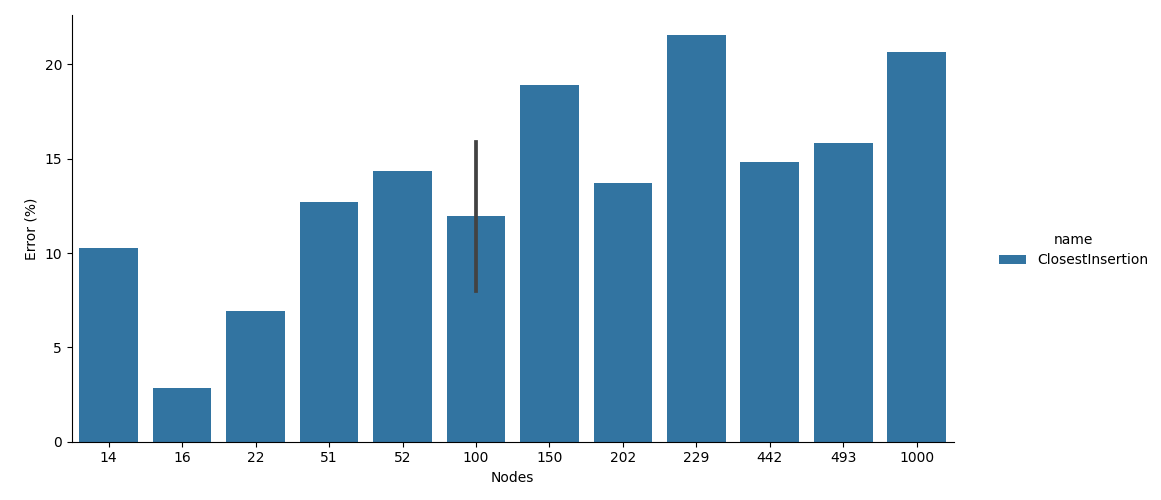
\includegraphics[width=0.9\textwidth]{./images/ClosestInsertion__approximation_error_.png}

    \caption{ClosestInsertion accuracy error scaling by nodes}
    \label{fig:closest-insertion-accuracy-error}
\end{figure}

\subsubsection{Osservazioni}

Data la netta dualità con FarthestInsertion, è doveroso analizzare
le differenze tra i due algoritmi. Dalla tabella 
\ref{table:closest-farthest-insertion-runtime-accuracy} 
e dal grafico \ref{fig:closest-farthest-insertion-accuracy-error}
è possibile notare che per quanto riguarda il runtime i due algoritmi
sono perfettamente alla pari, infatti minimizzare o massimizzare la
funzione $\delta (k, C)$ dal punto di vista del tempo di esecuzione
non comporta differenze. Dal punto di vista dell'errore di 
approssimazione invece FarthestInsertion riesce a fare mediamente
meglio di ClosestInsertion. Da sottolineare anche il fatto che 
FarthestInsertion riesce ad eliminare completamente l'errore di
approssimazione su istanze molto piccole.

\begin{figure}[H]
    \centering

    \begin{tabular}{lrrrrrr}
    \toprule
    \multicolumn{1}{c}{ } & \multicolumn{3}{c}{Closest Insertion} & \multicolumn{3}{c}{Farthest Insertion} \\
    \hline
    Instance & Solution &   Time (ms) &   Error (\%) & Solution &   Time (ms) &   Error (\%) \\
    \hline
    burma14.tsp   &     3664 &          35 &       10.26 &       3323 &          35 &        0    \\
    ulysses16.tsp &     7054 &          36 &        2.84 &       6859 &          35 &        0    \\
    ulysses22.tsp &     7499 &          36 &        6.93 &       7013 &          35 &        0    \\
    eil51.tsp     &      480 &          37 &       12.68 &        439 &          36 &        3.05 \\
    berlin52.tsp  &     8626 &          35 &       14.37 &       8118 &          36 &        7.64 \\
    kroA100.tsp   &    24661 &          38 &       15.88 &      23373 &          36 &        9.83 \\
    kroD100.tsp   &    22998 &          38 &        8    &      22577 &          36 &        6.03 \\
    ch150.tsp     &     7763 &          40 &       18.92 &       6864 &          41 &        5.15 \\
    gr202.tsp     &    45660 &          46 &       13.7  &      45211 &          46 &       12.58 \\
    gr229.tsp     &   163597 &          52 &       21.54 &     148324 &          52 &       10.19 \\
    pcb442.tsp    &    58297 &         142 &       14.81 &      56964 &         140 &       12.18 \\
    d493.tsp      &    40537 &         180 &       15.81 &      39506 &         176 &       12.87 \\
    dsj1000.tsp   & 22510610 &        1127 &       20.64 &   20599827 &        1125 &       10.4  \\
    \bottomrule
    \end{tabular}

    \caption{ClosestInsertion vs FarthestInsertion runtime and accuracy error}
    \label{table:closest-farthest-insertion-runtime-accuracy}
\end{figure}

\begin{figure}[H]
    \centering

    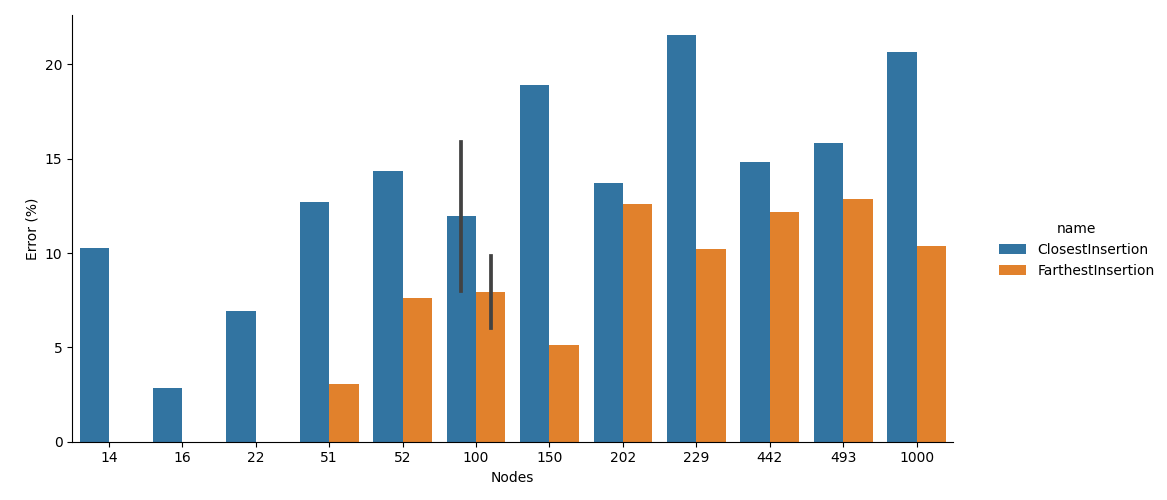
\includegraphics[width=0.9\textwidth]{./images/ClosestInsertion_vs_FarthestInsertion__approximation_error_.png}

    \caption{ClosestInsertion vs FarthestInsertion accuracy error scaling by nodes}
    \label{fig:closest-farthest-insertion-accuracy-error}
\end{figure}